\chapter{平衡常数与平衡移动}\label{ch:b2:equilibrium-shifts}

某合成氨工厂的转化器在约 \qty{450}{\celsius} 和
\qty{200}{bar} 下运行。室温下，\ce{N2 + 3H2 <=>
2NH3} 的平衡强烈偏向氨，以至于元素混合物原则上
几乎可以完全转化；然而工程师仍要加热，这会使
平衡逆向移动，再将其压缩至两百
个大气压，耗能巨大。其原因在于
反应能进行到何种程度与其进行得多快之间的折中。本章
将前几章的\omterm{def:b2:reaction-free-energy:gibbs-energy}{吉布斯自由能}转化为
本科一年级分册中的平衡常数，说明该常数如何随温度变化，
统计实验者可自由选择的条件数目，
并预测温度、压强或组成改变时平衡的
移动方向。

\begin{recall}
\Cref{ch:b2:reaction-free-energy}：演化判据 $\Delta_r G\,\dd\xi
\leq 0$ 与吉布斯–亥姆霍兹关系；
\cref{ch:b2:chemical-potential}：$\Delta_r G = \Delta_r G^\circ + RT\ln Q$。
本科一年级分册中的反应商 $Q = \prod_i a_i^{\nu_i}$，标准
平衡常数 $K^\circ$（即平衡时 $Q$ 的值）、质量作用定律和
判据“$Q < K^\circ$：正向进行”，均在那里作为
定律给出；进度表；一个或两个反应的最终状态。该册还
承诺在此说明合成氨和
三氧化硫的温度与压强的选择。
\end{recall}

\begin{omfigure}
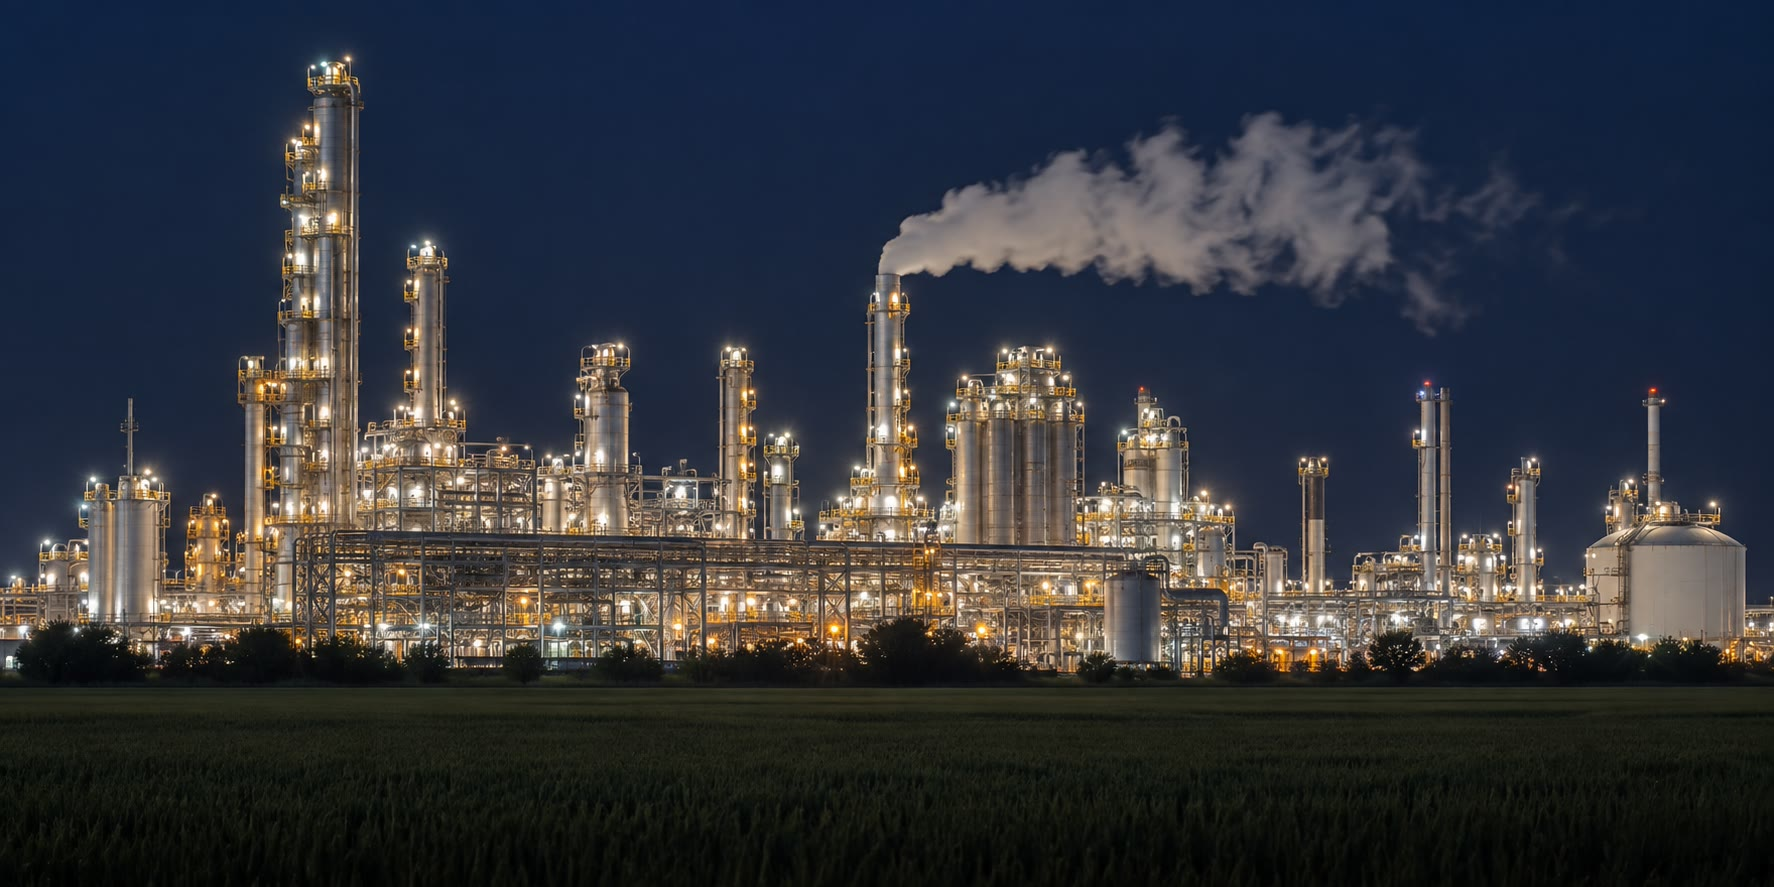
\includegraphics[width=0.7\linewidth]{images/book3/ai/b2-04-ammonia-plant.jpg}

{\small 夜晚的合成氨工厂。在其转化器中，氮气和氢气
在数百摄氏度和数百巴下流经铁催化剂；
这些条件的选择是周末问题的主题。}
\end{omfigure}

\section{由吉布斯自由能求平衡常数}

\begin{theorem}[标准平衡常数]\label{thm:b2:equilibrium-shifts:k-from-g}
平衡时 $\Delta_r G = 0$，且反应商取值为
\[
  K^\circ(T) = \exp\!\left(-\frac{\Delta_r G^\circ(T)}{RT}\right), \qquad
  \Delta_r G^\circ(T) = -RT\ln K^\circ(T) .
\]
它仅取决于温度。
\end{theorem}

\begin{proof}
由演化判据，$\Delta_r G = 0$ 即为平衡条件。
由 $\Delta_r G = \Delta_r G^\circ + RT\ln Q$
（见\cref{prop:b2:chemical-potential:delta-g-q}），平衡意味着 $\ln Q_{\text{平衡}}
= -\Delta_r G^\circ/(RT)$，仅是 $T$ 的函数，因 $\Delta_r G^\circ$ 亦如此。
\end{proof}

\begin{corollary}[本科一年级分册中的定律]\label{cor:b2:equilibrium-shifts:mass-action}
$\Delta_r G = RT\ln(Q/K^\circ)$。由此，$Q < K^\circ$ 的系统正向演化，
$Q > K^\circ$ 的系统逆向演化，$Q = K^\circ$ 的系统处于
平衡（即质量作用定律）。
\end{corollary}

\begin{proof}
将 $\Delta_r G^\circ = -RT\ln K^\circ$ 代入 $\Delta_r G = \Delta_r G^\circ
+ RT\ln Q$ 中，$\Delta_r G$ 的符号与 $\ln(Q/K^\circ)$ 相同，而
演化判据要求 $\Delta_r G\,\dd\xi \leq 0$。
\end{proof}

\begin{example}[\qty{298}{K} 时的三个常数]\label{ex:b2:equilibrium-shifts:constants}
合成氨，$\Delta_r G^\circ = \qty{-32.8}{kJ/mol}$：$K^\circ =
\exp(32\,800/(8.314 \times 298.15)) = \num{5.6e5}$（查表，取更多位数，
则得 \num{5.4e5}）。\ce{N2O4} 的解离，$\Delta_r G^\circ =
\qty{+4.7}{kJ/mol}$：$K^\circ = 0.15$。石灰石的分解，
$\Delta_r G^\circ = \qty{+130.4}{kJ/mol}$：$K^\circ = \num{1.5e-23}$，
而室温下石灰石上方二氧化碳的平衡压强
为 $\num{1.5e-23}$ 巴，几乎为零。$\Delta_r G^\circ$ 在 \qty{298}{K} 时每改变
\qty{5.7}{kJ/mol}，$K^\circ$ 即乘以或除以十。
% ledger: dfh:NH3_g, s0:NH3_g, janafG:NH3.298.15 (computed in figdata/bachelor-2/thermo-data.py and vant-hoff.py)
\end{example}

整个系统的\omterm{def:b2:reaction-free-energy:gibbs-energy}{吉布斯自由能}以“地貌”的形式显示了同样的结论：
它在平衡反应进度处取最低值，此处其斜率 $\Delta_r G$
为零。

\begin{omfigure}
\begin{tikzpicture}
\begin{axis}[
  width=0.7\linewidth, height=5.6cm, xmin=0, xmax=1, ymin=-2.2, ymax=5.2,
  axis x line=bottom, axis y line=left, xlabel={反应进度 $\xi$（摩尔）},
  ylabel={$G(\xi) - G(0)$ (\unit{kJ})},
  tick label style={font=\small}, label style={font=\small}, clip=false]
\addplot[omDef, very thick] table[x=xi, y=G] {figdata/out/bachelor-2-gibbs-extent.dat};
\draw[dotted] (axis cs:0.189,-2.2) -- (axis cs:0.189,-0.949);
\fill[omThm] (axis cs:0.189,-0.949) circle (1.6pt);
\node[omThm, anchor=west, font=\small] at (axis cs:0.21,-1.75) {平衡，$\xi = 0.189$};
\draw[dashed, gray] (axis cs:0,0) -- (axis cs:1,4.728);
\node[gray, font=\scriptsize, anchor=south east] at (axis cs:1,4.75) {$\xi\,\Delta_r G^\circ$};
\end{axis}
\end{tikzpicture}

{\small 封闭理想气体系统在 \qty{298}{K} 和
\qty{1}{bar} 下的\omterm{def:b2:reaction-free-energy:gibbs-energy}{吉布斯自由能}，从 \qty{1}{mol} 的 \ce{N2O4} 出发，随
\ce{N2O4 <=> 2NO2} 的反应进度而变。虽然 $\Delta_r G^\circ > 0$（虚线，纯组分），
两种气体混合使 $G$ 降低，最小值位于 $\xi =
0.189$ 处，此时 $Q = K^\circ = 0.15$。在其左侧，斜率 $\Delta_r G =
\partial G/\partial\xi$ 为负，在其右侧为正。}
% ledger: dfh:N2O4_g, s0:N2O4_g, dfh:NO2_g, s0:NO2_g (computed in figdata/bachelor-2/gibbs-extent.py)
\end{omfigure}

\section{温度：范托夫方程}

\begin{theorem}[范托夫方程]\label{thm:b2:equilibrium-shifts:vant-hoff}
\[
  \frac{\dd\ln K^\circ}{\dd T} = \frac{\Delta_r H^\circ(T)}{RT^2}
\]
（\emph{范托夫方程}\index{范托夫方程}）：吸热反应的
平衡常数随温度升高而增大，放热反应的
则随温度升高而减小。
\end{theorem}

\begin{proof}
由 $\ln K^\circ = -\Delta_r G^\circ/(RT)$ 出发，利用吉布斯–亥姆霍兹关系
（见\cref{prop:b2:reaction-free-energy:gibbs-helmholtz}），
\[
  \frac{\dd}{\dd T}\left(\frac{\Delta_r G^\circ}{T}\right) =
  -\frac{\Delta_r H^\circ}{T^2} ;
\]
两边除以 $-R$。
\end{proof}

\begin{proposition}[积分形式]\label{prop:b2:equilibrium-shifts:integrated}
若 $\Delta_r H^\circ$ 在 $T_1$ 与 $T_2$ 之间为常数，
（\omterm{def:b2:reaction-free-energy:ellingham-approximation}{埃林厄姆近似}），则
\[
  \ln\frac{K^\circ(T_2)}{K^\circ(T_1)} = -\frac{\Delta_r H^\circ}{R}\left(
  \frac{1}{T_2} - \frac{1}{T_1}\right),
\]
且 $\ln K^\circ$ 是一条斜率为 $-\Delta_r H^\circ/R$ 的直线，横坐标为
$1/T$.
\end{proposition}

\begin{proof}
对 $\dd\ln K^\circ = (\Delta_r H^\circ/R)\,\dd T/T^2$ 积分，注意到
$\dd T/T^2 = -\dd(1/T)$。
\end{proof}

\begin{omfigure}
\begin{tikzpicture}
\begin{axis}[
  width=0.72\linewidth, height=5.8cm, xmin=0.9, xmax=3.5, ymin=-19, ymax=15,
  axis x line=bottom, axis y line=left, xlabel={$1000/T$ (\unit{1/K})},
  ylabel={$\ln K^\circ$}, tick label style={font=\small},
  label style={font=\small}, clip=false]
\addplot[omThm, dashed, thick] table[x=invT, y=lnK] {figdata/out/bachelor-2-vant-hoff-a-line.dat};
\addplot[omDef, only marks, mark=*, mark size=1.8pt] table[x=invT, y=lnK] {figdata/out/bachelor-2-vant-hoff-a.dat};
\node[omDef, font=\scriptsize, anchor=west] at (axis cs:3.36,13.2) {\qty{298}{K}};
\node[omDef, font=\scriptsize, anchor=north west] at (axis cs:1.03,-15.3) {\qty{1000}{K}};
\node[omThm, font=\small, anchor=south east, align=right] at (axis cs:2.4,8) {斜率 $-\Delta_r H^\circ(298)/R$\\ $= +11\,050$ K};
\end{axis}
\end{tikzpicture}

{\small 表中数据给出 \ce{N2 + 3H2 <=> 2NH3} 的平衡常数（圆点，温度从 298 至
\qty{1000}{K}），虚线为取 \qty{298}{K} 时的 $\Delta_r H^\circ$ 所画的范托夫直线。
该反应为放热反应：$K^\circ$ 从
\num{5e5} 降至 \num{3e-7}。高温下各点落在直线下方：
$\Delta_r H^\circ$ 随 $T$ 升高而变得更负
（见\cref{ex:b2:reaction-enthalpy:kirchhoff}）。}
% ledger: janafG:NH3.298.15, janafG:NH3.400, janafG:NH3.500, janafG:NH3.600, janafG:NH3.700, janafG:NH3.800, janafG:NH3.900, janafG:NH3.1000, dfh:NH3_g (computed in figdata/bachelor-2/vant-hoff.py)
\end{omfigure}

\begin{method}[求另一温度下的平衡常数]\label{met:b2:equilibrium-shifts:k-at-t}
\begin{enumerate}
  \item 由 \qty{298}{K} 时的数据表，计算 $\Delta_r H^\circ$、$\Delta_r
        S^\circ$ 以及 $K^\circ(298)$。
  \item 可用积分形式的\omterm{thm:b2:equilibrium-shifts:vant-hoff}{范托夫方程}，或先计算
        $\Delta_r G^\circ(T) = \Delta_r H^\circ - T\Delta_r S^\circ$，再求
        $K^\circ(T)$：二者所用的近似相同。
  \item 若温度区间较宽或 $\Delta_r C_p^\circ$ 较大，宜采用表列的
        $\Delta_f G^\circ(T)$ 值；在 \qty{298}{K} 时误差为 \qty{5.7}{kJ/mol}
        （或在 \qty{700}{K} 时为 \qty{13}{kJ/mol}）即会使 $K^\circ$ 相差十倍。
\end{enumerate}
\end{method}

\begin{history}[雅各布斯·亨利库斯·范托夫]
\begin{minipage}[t]{0.2\linewidth}\vspace{0pt}
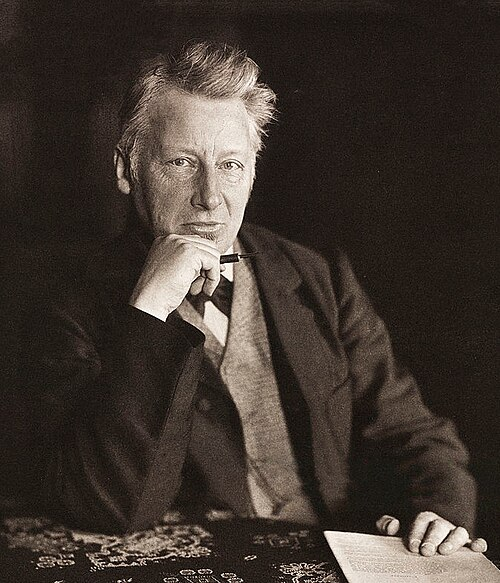
\includegraphics[width=\linewidth]{images/book3/vanthoff.jpg}
\end{minipage}\hfill
\begin{minipage}[t]{0.76\linewidth}\vspace{0pt}
雅各布斯·亨利库斯·范托夫（1852--1911）于 1884 年在其著作
《化学动力学研究》 中给出了
以他名字命名的温度与平衡常数之间的关系，次年又给出了
\cref{ch:b2:chemical-potential}中的\omterm{def:b2:chemical-potential:osmotic-pressure}{渗透压}定律；十年前他曾提出
四面体碳原子的假说。他获得了首届诺贝尔
化学奖（1901 年）。（照片由 N. Perscheid 摄于 1904 年：公有领域，
维基共享资源。）
\end{minipage}
\end{history}

\section{自由度}

实验者可以自由固定多少个强度量，
才能使平衡状态被完全确定？

\begin{definition}[自由度]\label{def:b2:equilibrium-shifts:variance}
\emph{独立强度变量}\index{独立强度变量}是处于平衡的系统的
一组强度量，
（温度、压强、各相中的摩尔分数），它们可以相互独立地选取，
且一经选定即可确定其余所有强度量。它们的个数称为该系统的
\emph{自由度}\index{自由度} $v$。
\end{definition}

\begin{theorem}[相律]\label{thm:b2:equilibrium-shifts:phase-rule}
对于 $n$ 种物种分布于 $\varphi$ 个相中、由 $r$ 个
独立平衡反应以及 $s$ 个强度量之间的附加关系相联系的系统，
这些关系由制备方式所确定（如化学计量进料、
电中性），
\[
  v = c + 2 - \varphi, \qquad c = n - r - s .
\]
\end{theorem}

\begin{proof}
强度变量有：$T$、$p$，以及每相中
$n$ 种物种的摩尔分数，它们之和为 1，故每相有 $n - 1$ 个自由变量，共计 $2 +
\varphi(n - 1)$ 个。关系式有：每种物种在各相之间处于平衡，
相间给出 $\varphi - 1$ 个\omterm{def:b2:chemical-potential:chemical-potential}{化学势}相等式（每种物种各一组），合计 $n(\varphi -
1)$ 个；每个反应给出 $Q = K^\circ(T)$，$r$ 个关系；另有 $s$
个附加关系。相减得：$v = 2 + \varphi(n - 1) - n(\varphi - 1) - r -
s = n - r - s + 2 - \varphi$。（某物种不在某相中时，
同时减少一个变量和一个关系。）
\end{proof}

\begin{method}[计算自由度]\label{met:b2:equilibrium-shifts:variance}
\begin{enumerate}
  \item 列出各物种及其所在的相，并数出 $n$ 与 $\varphi$
        （每种纯固体各为一个相；所有气体合为一个相）。
  \item 数出其中独立反应的个数 $r$。
  \item 数出附加关系的个数 $s$：处于化学计量比的物质的量关系
        （仅当该关系涉及同一相中的量时），
        离子溶液的电中性。
  \item $v = n - r - s + 2 - \varphi$.
\end{enumerate}
\end{method}

\begin{example}[三个自由度的计算]\label{ex:b2:equilibrium-shifts:variances}
石灰石置于封闭容器中，\ce{CaCO3(s) <=> CaO(s) + CO2(g)}：$n = 3$，$r =
1$，$\varphi = 3$（两种固体、一种气体）：$v = 1$。选定 $T$ 后，
二氧化碳的压强即已确定：$p = K^\circ(T)\,p^\circ$。气体混合物
由 \ce{N2}、\ce{H2} 与 \ce{NH3} 组成，处于平衡：$n = 3$，$r = 1$，$\varphi = 1$，$v
= 3$（$T$、$p$ 与一个组成变量）；若仅由氨出发，或由
化学计量比投料，\ce{N2} 与 \ce{H2} 之比为 1 : 3，$s = 1$，且
$v = 2$：给定 $T$ 与 $p$ 时组成即已确定，正如周末问题
所用。
\end{example}

\section{平衡移动}

\begin{definition}[平衡移动]\label{def:b2:equilibrium-shifts:shift}
处于平衡的体系受到扰动（温度的改变、
压强或某物质的量的改变）时，体系一般不再处于平衡，并
演化至新的平衡。称\emph{平衡移动}\index{平衡移动}
为正向（$\dd\xi > 0$，即反应向前进行），
否则为逆向。
\end{definition}

\begin{method}[预测平衡移动方向]\label{met:b2:equilibrium-shifts:predict-shift}
扰动刚发生后，计算（或估计）
$Q$ 与 $K^\circ$ 变化的符号。若此时 $Q < K^\circ$，则正向移动；若 $Q > K^\circ$，
则逆向移动；若等式仍成立，则不移动。
\end{method}

\begin{omfigure}
\begin{tikzpicture}[font=\small, >={Stealth}]
  \draw[->, thick] (0,0) -- (11,0) node[right] {$\ln Q$};
  \draw[omThm, thick] (5.5,0.25) -- (5.5,-0.25) node[below, align=center] {$\ln K^\circ$\\（$= \ln Q$ 之前）};
  \fill (5.5,0) circle (2pt);
  \draw[omDef, thick] (2.8,0.25) -- (2.8,-0.25) node[below] {$\ln Q$ 刚扰动后};
  \draw[->, omDef, very thick] (3.0,0.6) -- (5.2,0.6) node[midway, above] {正向移动};
  \draw[omProp, thick] (8.4,0.25) -- (8.4,-0.25) node[below] {$\ln Q$ 刚扰动后};
  \draw[->, omProp, very thick] (8.2,0.6) -- (5.8,0.6) node[midway, above] {逆向移动};
\end{tikzpicture}

{\small 扰动使 $Q$（温度改变时则为 $K^\circ$）发生移动；
体系随之移动，直至 $Q = K^\circ$ 再次成立：若 $Q$ 变得
过小则正向移动，过大则逆向移动。}
\end{omfigure}

\begin{proposition}[温度]\label{prop:b2:equilibrium-shifts:temperature}
恒压下，升高温度使平衡沿吸热
方向移动（若 $\Delta_r H^\circ > 0$，则为正向），降低温度则使其沿
放热方向移动。
\end{proposition}

\begin{proof}
组成与压强固定时，$Q$ 不随 $T$ 改变（对理想
体系而言）；由范托夫关系，$K^\circ$ 随 $T$ 增大（当 $\Delta_r H^\circ >
0$ 时）。刚使 $T$ 升高后，$Q < K^\circ$，平衡正向移动。
\end{proof}

\begin{proposition}[压强]\label{prop:b2:equilibrium-shifts:pressure}
恒温、组成不变时，升高气相平衡体系的总压，
平衡向使气体分子数减少的方向移动（
$\Delta\nu_{\text{气体}} < 0$ 时为正向）。若 $\Delta\nu_{\text{气体}}
= 0$，则压强对平衡无影响。
\end{proposition}

\begin{proof}
设 $p_i = x_ip$，$Q = \prod_i x_i^{\nu_i}\,(p/p^\circ)^{\Delta\nu_{\text{气体}}}$：
组成不变时，升高 $p$ 使 $Q$ 乘以
$(p'/p)^{\Delta\nu_{\text{气体}}}$，该因子 $< 1$（当 $\Delta\nu_{\text{气体}} <
0$ 时）。于是 $Q < K^\circ$：正向。凝聚相无贡献。
\end{proof}

\begin{proposition}[加入组分或惰性气体]\label{prop:b2:equilibrium-shifts:adding}
在气相平衡中加入少量气态组分 $j$，
使 $\ln Q$ 改变
\[
  \left(\frac{\partial\ln Q}{\partial n_j}\right) = \frac{\nu_j}{n_j} -
  \frac{\Delta\nu_{\text{气体}}}{n_{\text{总}}}\ \ \text{ 恒定 } T, p ;
  \qquad \frac{\nu_j}{n_j}\ \ \text{ 恒定 } T, V .
\]
加入惰性气体在恒容时无影响，在恒压时
相当于降低压强。
\end{proposition}

\begin{proof}
在 $T$、$p$ 恒定时：$Q = \prod_i n_i^{\nu_i}\,(p/(p^\circ n_{\text{总}}))^{
\Delta\nu_{\text{气体}}}$，其关于 $n_j$ 的对数导数为
$\nu_j/n_j - \Delta\nu_{\text{气体}}/n_{\text{总}}$（对惰性
气体，$\nu_j = 0$，第一项为零）。在 $T$、$V$ 恒定时：$p_i = n_iRT/V$，$Q = \prod_i n_i^{
\nu_i}\,(RT/(p^\circ V))^{\Delta\nu_{\text{气体}}}$，其导数
仅为 $\nu_j/n_j$。
\end{proof}

\begin{remark}[加入反应物反而使反应逆向进行]\label{rem:b2:equilibrium-shifts:paradox}
在合成氨中，$\nu(\ce{N2}) = -1$，且 $\Delta\nu_{\text{气体}} = -2$：
在 $T$、$p$ 恒定时加入氮气，$\ln Q$ 改变 $-1/n_{\ce{N2}} +
2/n_{\text{总}}$，当 $x(\ce{N2}) > 1/2$ 时为正。在
已富含氮的混合物中，再加氮气会将氢气稀释得很厉害，
以致氨发生分解。“加入反应物使平衡正向移动”这一规则
在恒容时可靠，在恒压时则不一定成立。
\end{remark}

\begin{proposition}[勒夏特列原理]\label{prop:b2:equilibrium-shifts:le-chatelier}
上述各命题可归结为\emph{勒夏特列原理}\index{勒夏特列原理}：
处于平衡状态的系统，若温度或压强受到扰动，
则向着抵消该扰动的方向移动（受热时
吸收热量，受压缩时
减小气体体积）。
\end{proposition}

\begin{proof}
这实际上是重述\cref{prop:b2:equilibrium-shifts:temperature}
（吸热方向吸收热量）与\cref{prop:b2:equilibrium-shifts:pressure}
（在相同的 $T$、$p$ 下，气体分子数较少者占据较小体积）。对于恒压下加入物质的情形，
该原理并不可靠
（见\cref{rem:b2:equilibrium-shifts:paradox}）：应计算 $Q$。
\end{proof}

\begin{remark}[平衡何时终止]\label{rem:b2:equilibrium-shifts:rupture}
移动的结果可能不是建立新的平衡，而是某一相消失。
在密闭容器中加热石灰石，它会分解，直至 $p(\ce{CO2}) =
K^\circ(T)\,p^\circ$；若其量不足以达到该压强，则会全部消失，此时 $Q$ 始终小于 $K^\circ$：
系统永久地处于非平衡状态，
正如本科一年级分册已观察到的那样。
\end{remark}

\begin{history}[亨利·勒夏特列]
\begin{minipage}[t]{0.2\linewidth}\vspace{0pt}
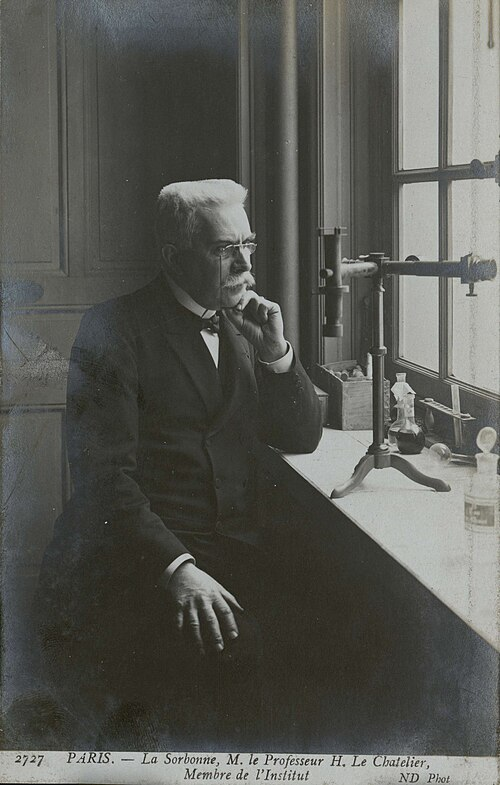
\includegraphics[width=\linewidth]{images/book3/lechatelier.jpg}
\end{minipage}\hfill
\begin{minipage}[t]{0.76\linewidth}\vspace{0pt}
亨利·勒夏特列（1850--1936）是一位采矿工程师兼化学家，
研究水泥、冶金与高温测量，于 1884 年提出了以其命名的“\omterm{def:b2:equilibrium-shifts:shift}{平衡移动}定律”。
约在 1901 年，他还曾尝试在加压条件下由氮气与氢气直接合成氨，
但其装置发生爆炸，实验因此中止。
（照片：作者不详，CC BY-SA 4.0，维基共享资源。）
\end{minipage}
\end{history}

\section{合成的优化}

\subsection*{氨}

\begin{omfigure}
\begin{tikzpicture}
\begin{axis}[
  width=0.78\linewidth, height=6.2cm, xmin=500, xmax=1000, ymin=0, ymax=0.9,
  axis x line=bottom, axis y line=left, xlabel={$T$ (K)},
  ylabel={\ce{NH3} 的平衡摩尔分数},
  tick label style={font=\small}, label style={font=\small}, clip=false]
\addplot[omThm, very thick] table[x=T, y=p300] {figdata/out/bachelor-2-vant-hoff-b.dat};
\addplot[omDef, very thick] table[x=T, y=p200] {figdata/out/bachelor-2-vant-hoff-b.dat};
\addplot[omProp, very thick] table[x=T, y=p50] {figdata/out/bachelor-2-vant-hoff-b.dat};
\addplot[black!60, very thick] table[x=T, y=p1] {figdata/out/bachelor-2-vant-hoff-b.dat};
\node[omThm, font=\scriptsize, anchor=south west] at (axis cs:600,0.70) {300 巴};
\node[omDef, font=\scriptsize, anchor=north east] at (axis cs:612,0.52) {200 巴};
\node[omProp, font=\scriptsize, anchor=north east] at (axis cs:578,0.30) {50 巴};
\node[black!60, font=\scriptsize, anchor=south west] (onebar) at (axis cs:520,0.13) {1 巴};
\draw[black!60] (onebar.south west) -- (axis cs:512,0.075);
\draw[dotted] (axis cs:723,0) -- (axis cs:723,0.253);
\fill[omDef] (axis cs:723,0.253) circle (1.6pt);
\end{axis}
\end{tikzpicture}

{\small 由 1 : 3 的氮气与氢气混合物（视为理想气体）计算得到的氨平衡摩尔分数，
随温度变化，共四条压强曲线，由表列\omterm{def:b2:reaction-free-energy:gibbs-energy}{吉布斯自由能}算出。
压强升高使其增大，温度升高使其减小；
圆点标出 \qty{723}{K} 与 \qty{200}{bar} 的位置。}
% ledger: janafG:NH3.500, janafG:NH3.600, janafG:NH3.700, janafG:NH3.800, janafG:NH3.900, janafG:NH3.1000 (computed in figdata/bachelor-2/vant-hoff.py)
\end{omfigure}

合成反应为放热反应，且将四分子气体转化为两分子：由上述命题可知，
低温和高压有利于氨的生成。
在 \qty{1}{bar} 与室温下，平衡几乎完全偏向产物一侧，
但反应根本无法进行：氮分子的三键只有在催化剂作用下才会断裂，
而铁催化剂仅在数百度时才有效。
因此，工厂的做法是：
\begin{itemize}
  \item 温度应足够高以保证反应速率，且尽可能低于催化剂所允许的温度
        （约 \qty{700}{K}）；
  \item 采用高压以弥补因温度而损失的产率，但受限于
        压缩成本与厚壁容器；
  \item 设置\omterm{def:b2:equilibrium-shifts:single-pass}{循环}：离开转化器的气体先被冷却，氨凝结并被移出，
        未转化的气体与新鲜原料一同\omterm{def:b2:equilibrium-shifts:single-pass}{循环}回用；
        另设少量\omterm{def:b2:equilibrium-shifts:single-pass}{驰放}，以排出否则会不断积累的氩气
        与甲烷。
\end{itemize}

\begin{definition}[单程转化率、循环与驰放]\label{def:b2:equilibrium-shifts:single-pass}
在带有循环的过程中，\emph{单程转化率}\index{单程转化率}
是指一种反应物在经过反应器一次时被转化的比例；
未转化的部分与产物分离后，
作为\emph{循环}\index{循环}返回反应器入口；
\emph{驰放}\index{驰放}是指从循环中连续抽出的一小股气流，
用以防止惰性组分不断积累。
\end{definition}

\begin{omfigure}
\begin{tikzpicture}[font=\small, >={Stealth}, box/.style={draw, thick, rounded corners=2pt, minimum width=2.1cm, minimum height=1.0cm, align=center, fill=white}]
  \node[box] (comp) at (0,0) {压缩机};
  \node[box] (conv) at (3.6,0) {转化器 \\ （催化剂）};
  \node[box] (cond) at (7.2,0) {冷却器与 \\ 分离器};
  \draw[->, thick] (-3.9,0) -- (comp) node[pos=0.0, above right] {新鲜 \ce{N2 + 3H2}};
  \draw[->, thick] (comp) -- (conv);
  \draw[->, thick] (conv) -- (cond);
  \draw[->, thick, omDef] (cond.south) -- ++(0,-1.0) node[below] {液氨};
  \draw[->, thick, omThm] (cond.north) -- ++(0,0.9) -| (comp.north);
  \node[omThm, above] at (2.6,1.4) {循环（未转化的气体）};
  \draw[->, thick, black!60] (6.1,1.4) -- (6.1,2.1) node[above] {驰放};
\end{tikzpicture}

{\small 合成氨\omterm{def:b2:equilibrium-shifts:single-pass}{循环}。每一次通过仅转化了一部分气体；氨被冷凝分离，
其余气体经再压缩后与新鲜原料一同送回。
\omterm{def:b2:equilibrium-shifts:single-pass}{驰放}用以排出不参与反应的氩气与甲烷，
防止其累积。}
\end{omfigure}

\begin{history}[哈伯与博施]
\begin{minipage}[t]{0.15\linewidth}\vspace{0pt}
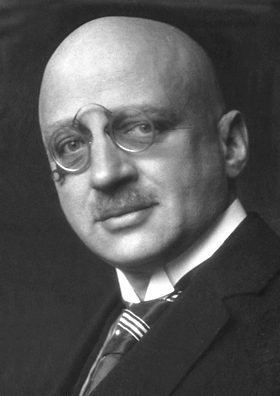
\includegraphics[width=\linewidth]{images/book3/haber.png}
\end{minipage}\hspace{0.01\linewidth}%
\begin{minipage}[t]{0.15\linewidth}\vspace{0pt}
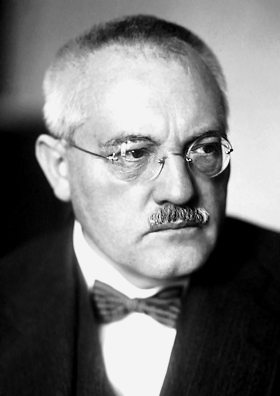
\includegraphics[width=\linewidth]{images/book3/bosch.jpg}
\end{minipage}\hfill
\begin{minipage}[t]{0.66\linewidth}\vspace{0pt}
弗里茨·哈伯（1868--1934）在加压下测定了氨的平衡，
并于 1909 年使其从实验室转化器中连续流出，经
锇催化剂。卡尔·博施（1874--1940）将其发展为工业生产，
所用钢制容器可耐受加压下的热氢，并采用廉价的铁
催化剂；第一座工厂于 1913 年投产。哈伯于
1918 年获诺贝尔奖，博施于 1931 年获奖。（照片：诺贝尔基金会肖像，公有领域，
维基共享资源。）
\end{minipage}
\end{history}

\subsection*{三氧化硫}

在接触法中，\ce{2SO2(g) + O2(g) <=> 2SO3(g)}（$\Delta_r H^\circ =
\qty{-197.8}{kJ/mol}$，对所写方程而言）；反应在氧化钒催化剂上进行，
该催化剂仅在高温下有活性，反应分若干段绝热床进行。
每段床内放出的热使温度升高，从而降低 $K^\circ$；转化
在气体到达平衡曲线时即停止。床间冷却使
气体回到平衡允许进一步转化的温度。
% ledger: dfh:SO2_g, dfh:SO3_g

\begin{omfigure}
\begin{tikzpicture}
\begin{axis}[
  width=0.72\linewidth, height=6.4cm, xmin=600, xmax=900, ymin=0, ymax=1.08,
  axis x line=bottom, axis y line=left, xlabel={$T$ (K)},
  ylabel={\ce{SO2} 的转化率}, tick label style={font=\small},
  label style={font=\small}, clip=false]
\addplot[black, very thick] table[x=T, y=X] {figdata/out/bachelor-2-vant-hoff-c.dat};
\addplot[omThm, thick] table[x=T, y=X] {figdata/out/bachelor-2-vant-hoff-bed1.dat};
\addplot[omThm, thick] table[x=T, y=X] {figdata/out/bachelor-2-vant-hoff-bed2.dat};
\addplot[omThm, thick] table[x=T, y=X] {figdata/out/bachelor-2-vant-hoff-bed3.dat};
\draw[->, omDef, thick] (axis cs:892.8,0.676) -- (axis cs:712,0.676);
\draw[->, omDef, thick] (axis cs:784.4,0.924) -- (axis cs:712,0.924);
\node[font=\scriptsize, anchor=south west] at (axis cs:860,0.84) {平衡};
\node[omThm, font=\scriptsize, anchor=west] at (axis cs:800,0.24) {第 1 段（绝热）};
\node[omDef, font=\scriptsize, anchor=south] at (axis cs:800,0.68) {冷却};
\end{axis}
\end{tikzpicture}

{\small \ce{SO2} 转化为 \ce{SO3} 的平衡转化率随温度的变化
（黑线），模型进料为 \qty{10}{\percent} \ce{SO2}、\qty{11}{\percent}
\ce{O2}，总压 \qty{1}{bar}，并给出气体经三段绝热床的路径
（红线，随反应放热而升温），段间经冷却
（蓝线）。}
% ledger: janafG:SO2.600, janafG:SO2.700, janafG:SO2.800, janafG:SO2.900, janafG:SO3.600, janafG:SO3.700, janafG:SO3.800, janafG:SO3.900 (computed in figdata/bachelor-2/vant-hoff.py; feed and adiabatic rise are model values)
\end{omfigure}

\section{练习}

\begin{exercise}[$\star$]\label{exo:b2:equilibrium-shifts:1}
计算 \qty{298}{K} 时 $K^\circ$ 的值，其中反应的 $\Delta_r G^\circ =
\qty{-32.8}{kJ/mol}$，再求 $\Delta_r G^\circ = \qty{+32.8}{kJ/mol}$ 时的值。
$\Delta_r G^\circ$ 需作怎样的改变，方能使 $K^\circ$ 变为原来的 100 倍？
\end{exercise}

\begin{exercise}[$\star$]\label{exo:b2:equilibrium-shifts:2}
对氨的合成反应，$K^\circ(298) = \num{5.4e5}$，且 $\Delta_r H^\circ =
\qty{-91.9}{kJ/mol}$。试估算 \qty{400}{K} 时的 $K^\circ$，
用积分形式的\omterm{thm:b2:equilibrium-shifts:vant-hoff}{范托夫方程}计算；表中给出的值为 35.6。
\end{exercise}

\begin{exercise}[$\star$]\label{exo:b2:equilibrium-shifts:3}
求下列各体系的\omterm{def:b2:equilibrium-shifts:variance}{自由度}：（a）与其蒸气平衡的液态水；
（b）封闭容器中的 \ce{CaCO3(s) <=> CaO(s) + CO2(g)}；（c）平衡时的 \ce{N2}、
\ce{H2}、\ce{NH3}，原料配比任意；（d）\ce{C(s) + H2O(g) <=>
CO(g) + H2(g)}。
\end{exercise}

\begin{exercise}[$\star$]\label{exo:b2:equilibrium-shifts:4}
对 \ce{N2O4(g) <=> 2NO2(g)}，$\Delta_r H^\circ > 0$。判断在
恒压升温、恒温压缩及恒容加入氩气时，
平衡分别向哪个方向移动？
\end{exercise}

\begin{exercise}[$\star\star$]\label{exo:b2:equilibrium-shifts:5}
对 \ce{N2(g) + O2(g) <=> 2NO(g)}，$\Delta_r H^\circ = \qty{180.6}{kJ/mol}$，
$\Delta_r S^\circ = \qty{24.8}{J/(K.mol)}$。计算 $K^\circ$ 在 \qty{298}{K}
和 \qty{2000}{K} 时的值（取\omterm{def:b2:reaction-free-energy:ellingham-approximation}{埃林厄姆近似}），并求空气中的
\ce{NO} 的摩尔分数（$x(\ce{N2}) = 0.78$，$x(\ce{O2}) = 0.21$，消耗甚少）
在 \qty{2000}{K} 平衡时的值。为何热机会生成这种污染物，
又为何它在冷却后的废气中仍会残留？
\end{exercise}

\begin{exercise}[$\star\star$]\label{exo:b2:equilibrium-shifts:6}
液相中的酯化反应 $\mathrm{A + B \rightleftharpoons E + W}$
其 $K^\circ = 4.0$（活度取为摩尔分数）。从
以 \qty{1.0}{mol} 酸 A 为起点，求醇 B 为 \qty{1.0}{mol} 时生成酯的物质的量，
醇 B 为 \qty{3.0}{mol} 时的情形。结合 $Q$ 与 $K^\circ$ 说明，为何将生成的水随生随移，
就能使反应进行完全。
\end{exercise}

\begin{exercise}[$\star\star$]\label{exo:b2:equilibrium-shifts:7}
在 \qty{298}{K}、\qty{1}{bar} 下，\ce{N2O4 <=> 2NO2} 的 $K^\circ = 0.148$。
求 \qty{1}{mol} \ce{N2O4} 的解离度。随后
在总压恒定下加入 \qty{1}{mol} 氩气，求新的
解离度，并予以解释。若在恒容下加入氩气，
结果又将如何？
\end{exercise}

\begin{exercise}[$\star\star$]\label{exo:b2:equilibrium-shifts:8}
氯化铵通过解离而升华，\ce{NH4Cl(s) <=> NH3(g) +
HCl(g)}。求气体仅由固体分解生成时以及
加入了一些氨时的\omterm{def:b2:equilibrium-shifts:variance}{自由度}，并说明两种情形对实验者各意味着什么。
\end{exercise}

\begin{exercise}[$\star\star$]\label{exo:b2:equilibrium-shifts:9}
表中给出合成氨在 \qty{500}{K} 时 $K^\circ = 0.0993$，
在 \qty{600}{K} 时 $K^\circ = \num{1.72e-3}$。由此求该区间内的 $\Delta_r H^\circ$，
并与 \qty{298}{K} 时的值比较。
\end{exercise}

\begin{exercise}[$\star\star\star$]\label{exo:b2:equilibrium-shifts:10}
证明\cref{rem:b2:equilibrium-shifts:paradox}中的反例：写出
以物质的量和总压表示的合成氨 $Q$，
计算 $\partial\ln Q/\partial n(\ce{N2})$（$T$ 与 $p$ 恒定），
并求使加入氮气后平衡逆向移动的 $x(\ce{N2})$ 所需满足的条件。
恒容下是否也会出现同样的情况？
\end{exercise}

\begin{exercise}[$\star\star\star$]\label{exo:b2:equilibrium-shifts:11}
石灰石在空的封闭容器中被加热至 \qty{1100}{K}，容器体积为
\qty{10.0}{L}，其分解反应的 $\Delta_r G^\circ = \qty{1.62}{kJ/mol}$，
（见\cref{ch:b2:reaction-free-energy}）。计算 $K^\circ$ 及
二氧化碳的平衡压强。求
\qty{0.050}{mol} 与 \qty{0.200}{mol} 石灰石各自的最终状态。
\end{exercise}

\begin{exercise}[$\star\star\star$]\label{exo:b2:equilibrium-shifts:12}
读出接触法图中各床层出口处的转化率与温度，
解释为何单个绝热床层无论多长，
在此进料下转化率都不能超过约 68\,\%，
并说明为何应在床层之间冷却气体而非使催化剂全程保持低温，以及
限制末床层转化率的因素是什么。
\end{exercise}

\section{问题：氨循环}

\begin{problem}[{周末问题——合成氨反应的平衡常数
及其温度依赖关系，转化器条件下的组成，
压强、温度与惰性气体引起的移动，以及
循环}]
\label{pb:b2:equilibrium-shifts:1}
氨由化学计量比的原料按 \ce{N2(g) + 3H2(g) <=> 2NH3(g)} 制得。
数据：在 \qty{298.15}{K} 时，$\Delta_f H^\circ(\ce{NH3}) = \qty{-45.94}{kJ/mol}$，
$S^\circ_m$（\unit{J/(K.mol)}）\ce{NH3} 为 192.77，\ce{N2} 为 191.61，\ce{H2} 为 130.68；
表中给出 \qty{700}{K} 时 $\Delta_f G^\circ(\ce{NH3}) = \qty{+27.19}{kJ/mol}$，
在 \qty{800}{K} 时为 \qty{+38.66}{kJ/mol}。气体为理想气体；
取 $R = \qty{8.314}{J/(K.mol)}$。
% ledger: dfh:NH3_g, s0:NH3_g, s0:N2_g, s0:H2_g, janafG:NH3.700, janafG:NH3.800

\medskip
\noindent\textbf{第一部分——平衡常数。}
\begin{enumerate}
  \item 求 $\Delta_r H^\circ$、$\Delta_r S^\circ$ 与 $\Delta_r G^\circ$，
        在 \qty{298}{K} 时的值，以及 $K^\circ(298)$。
  \item 由表中数据求 \qty{700}{K} 与 \qty{800}{K} 时的 $K^\circ$。
  \item 由这两个值求 \qty{700}{K} 至
        \qty{800}{K} 区间内的平均 $\Delta_r H^\circ$，并与第 1 小题比较。
  \item 由两个表值，利用\omterm{thm:b2:equilibrium-shifts:vant-hoff}{范托夫方程}，
        估算 $K^\circ(\qty{723}{K})$。
  \item 用\omterm{def:b2:reaction-free-energy:ellingham-approximation}{埃林厄姆近似}求 $K^\circ(\qty{723}{K})$，
        由 \qty{298}{K} 时的数据计算，并讨论其差异。
\end{enumerate}

\medskip
\noindent\textbf{第二部分——转化器中的平衡。}
\begin{enumerate}[resume]
  \item 以 \qty{1}{mol} \ce{N2} 与 \qty{3}{mol} \ce{H2} 为原料，写出
        反应进度为 $\xi$ 时的各物质的量及总物质的量。
  \item 设 $x$ 为氨的摩尔分数，证明
        \ce{N2} 与 \ce{H2} 的摩尔分数分别为 $(1-x)/4$ 与 $3(1-x)/4$。
  \item 证明 $\dfrac{x}{(1-x)^2} = \dfrac{\sqrt{27}}{16}\,\dfrac{p}{p^\circ}\,
        \sqrt{K^\circ}$。
  \item 求 \qty{723}{K}、\qty{1}{bar} 下的 $x$。
  \item 求 \qty{723}{K}、\qty{200}{bar} 下的 $x$。
  \item 计算体系的\omterm{def:b2:equilibrium-shifts:variance}{自由度}，并解释为何 $T$ 与 $p$ 可以
        确定组成。
\end{enumerate}

\medskip
\noindent\textbf{第三部分——\omterm{def:b2:equilibrium-shifts:shift}{平衡移动}。}
\begin{enumerate}[resume]
  \item 不经计算，判断压强升高时平衡向哪个方向移动，
        温度升高时又向哪个方向移动？
  \item 氩气随制取氮气所用的空气一同进入体系。恒定总压下，
        其存在如何使\omterm{def:b2:equilibrium-shifts:shift}{平衡移动}？
  \item 某平衡混合物中 $x(\ce{N2}) = 0.30$。
        在 $T$ 与 $p$ 恒定下加入少量氮气，平衡会正向还是逆向移动？
  \item 在恒容下，结论是否改变？
  \item 气体返回转化器之前，先将其中的氨冷凝分离，
        这对转化器入口处的 $Q$ 有何影响？
\end{enumerate}

\medskip
\noindent\textbf{第四部分——\omterm{def:b2:equilibrium-shifts:single-pass}{循环}。}
\begin{enumerate}[resume]
  \item 离开转化器的气体中氨的含量为 \qty{18}{\percent}，低于
        平衡值。实际转化器为何达不到
        平衡？
  \item 计算与
        $x(\ce{NH3}) = 0.18$ 相对应、由化学计量比原料出发的氢气\omterm{def:b2:equilibrium-shifts:single-pass}{单程转化率}。
  \item 未反应的气体\omterm{def:b2:equilibrium-shifts:single-pass}{循环}使用。稳态运行时，单位时间内有 \qty{1.00}{mol}
        新鲜 \ce{N2} 进入体系，问单位时间内离开的氨有多少，
        单位时间内有多少氮气通过转化器？
  \item 为何必须从\omterm{def:b2:equilibrium-shifts:single-pass}{循环}气中\omterm{def:b2:equilibrium-shifts:single-pass}{驰放}少量气体？
  \item 为何不在 \qty{500}{K} 下运行，
        虽然那里的平衡要有利得多？
  \item 在理想气体模型下，给出化学计量比原料在 \qty{723}{K}、
        \qty{200}{bar} 下氨的平衡摩尔分数。
\end{enumerate}
\end{problem}
